%\begin{frame}{Notre approche}
%Repérage des concepts dans les deux corpus en se basant sur le poids de leur apparition
%\begin{table}[!ht]
%\footnotesize
%\begin{tabularx}{\textwidth}{>{\setlength\hsize{1\hsize}\setlength\linewidth{\hsize}}X>{\setlength\hsize{1\hsize}\setlength\linewidth{\hsize}}X>{\setlength\hsize{1\hsize}\setlength\linewidth{\hsize}}X}
%\hline
%\rowcolor{blue!10}
%\multicolumn{3}{c}{Mesures de pondération}\\
%\textsc{TF-IDF} & \textsc{BM25} & \textsc{BERT} \\
%\hline
%\begin{itemize}
%    \item évalue l’importance d’un terme contenu dans
%un document relativement à un corpus plus
%large 
%    \item récompense la fréquence des
%termes et pénalise la fréquence des documents 
%\end{itemize}
%
%&
%\begin{itemize}
%    \item amélioration de \textsc{TF-IDF} 
%    \item traite les longs documents et les problèmes liés à la saturation des termes
%\end{itemize}
% &
% \begin{itemize}
%     \item modèle pré-entraîné sur de gros corpus (apprentissage non-supervisé, architecture des transformeurs)
%     \item apprend des représentations de mots et de phrases (contexte + sémantique)
%     % \item architecture des transformeurs (réseau de neurones utilisé pour le TAL)
% \end{itemize}
%\end{tabularx}
%\end{table}
%\end{frame}
\begin{frame}{OBVIE -- corpus Charcot\footnote{\url{https://obtic.huma-num.fr/obvie/charcot/?view=corpus}}}
\danger{} impossible de quantifier l'importance des phrasèmes
\begin{figure}[!h]
    \centering
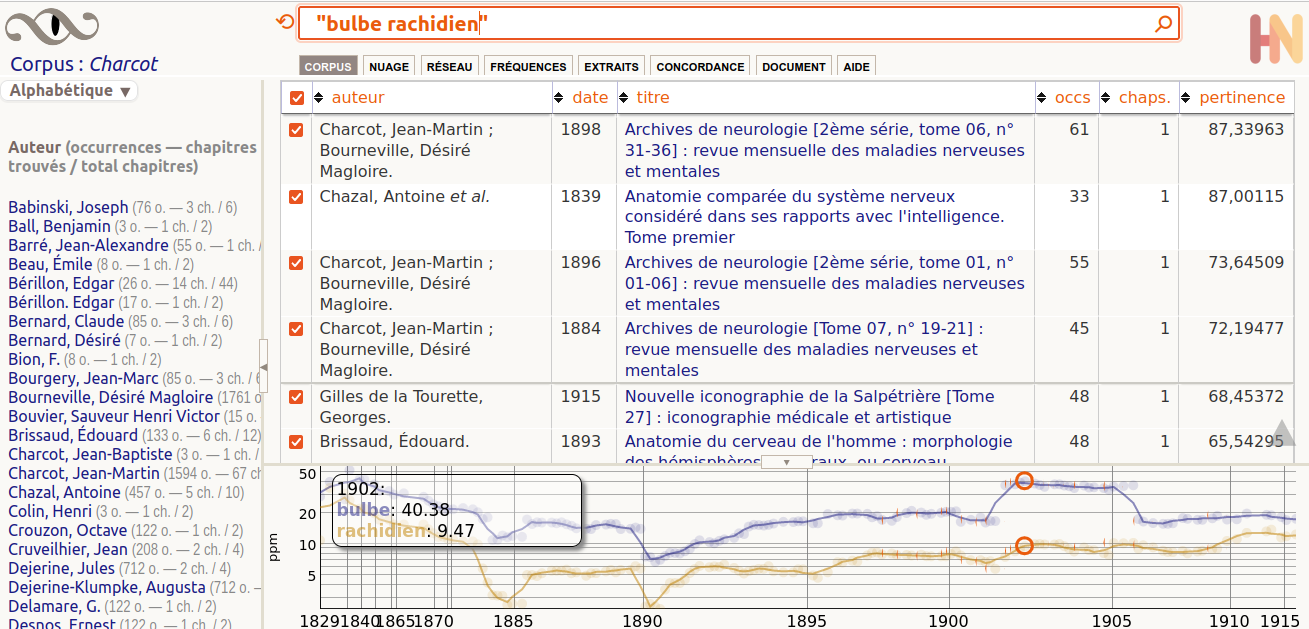
\includegraphics[width=90mm,scale=0.5]{pic/bulbe_rachidien.png}
    \caption{Distribution d'occurrences des tokens avec la frise chronologique pour ceux constituant l'expression \textit{bulbe rachidien}.}
    \label{fig:my_label}
\end{figure}
% citations directes (\cite{manjavacas2019})
\end{frame}

\begin{frame}{Liste des concepts médicaux}
    Extraction des termes ou des expressions popularisés par Charcot (\textit{hystérie}, \textit{sclérose latérale amyotrophique} etc.)
    \begin{itemize}
        \item index d’une édition des œuvres complètes de Charcot\footnote{\cite{charcot1890oeuvres}}
        \item sans les termes génériques (\textit{os, \textit{cerveau}, etc.})
        \item prise en compte des formes singulier / pluriel (regex)
    \end{itemize}
\end{frame}

\begin{frame}{Intensification du lexique
de Charcot dans le corpus \og{}Autres\fg}
\begin{figure}[!h]
    \centering
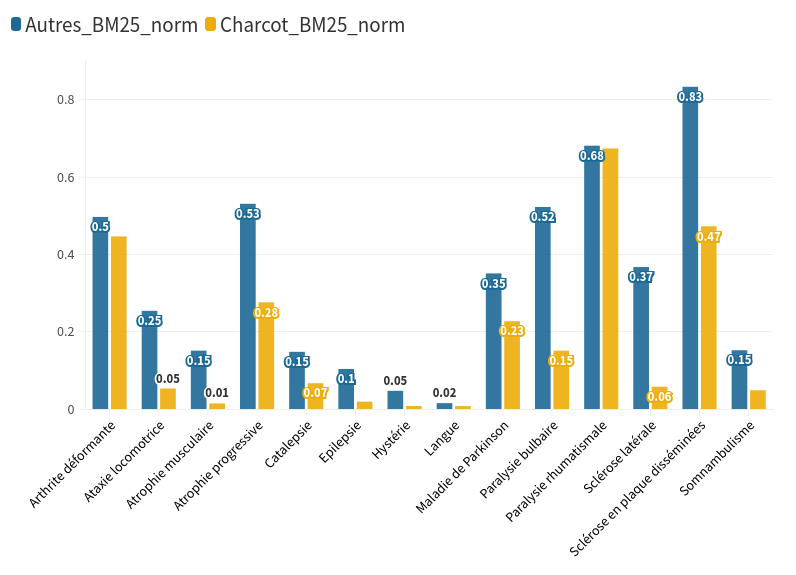
\includegraphics[width=94mm,scale=0.5]{pic/Charcot_Autres_250523.png}
    \caption{Pertinence des concepts dans les deux corpus (BM25).}
    \label{fig:my_label}
\end{figure}
\end{frame}

\begin{frame}{\textsc{TF-IDF}}
(angl. \textit{term frequency-inverse document frequency})\medskip

\color{deepblue}
Mesure pour quantifier l'importance ou la pertinence des représentations lexicales (mots, phrases, lemmes$\dots$) dans un document parmi une collection de documents (corpus).
\begin{itemize}
\item \textbf{TF} : fréquence d'un terme particulier par rapport au document.
\item \textbf{IDF} : calcule à quel point un terme est courant (ou rare) dans le corpus
\begin{itemize}
\item pénalise des termes fréquents et récompense les termes peu fréquents (considérés comme plus discriminants)
\end{itemize}
\end{itemize}
\end{frame}

\begin{frame}{\textsc{BM-25}}
(angl. \textit{best match} 25)\medskip

\color{deepblue}{Modèle de classement basé sur des termes qui vise à fournir des résultats de recherche précis et pertinents en classant les documents en fonction de la fréquence de leurs termes et de leur longueur.}

\begin{enumerate}
\item TF
\item IDF
\item normalisation de la longueur des documents
\item saturation des termes de requête
\end{enumerate}
\medskip

\color{deepgreen}{TF-IDF et BM25 sont les mesures couramment utilisées dans le domaine de recherche d'information (angl. \textit{information retrieval})}

\end{frame}

\begin{frame}{\textsc{BERT}}
\cite{vaswani2021}
    \begin{itemize}
        \item plongements lexicaux et des
mécanismes d’attention
        \item modèle \texttt{bert-base-multilingual-cased}
    \end{itemize}

\begin{table}[]
\begin{tabular}{ll}
\hline
Corpus « Charcot »             & Corpus « Autres » \\
\hline
diplopie (0,92)                & préambule (0,47)  \\
myélite partielle (0,91)       & délire (0,47)     \\
état de mal épileptique (0,91) & miracle (0,47)   \\
paralysie labio-glosso-laryngée (0,91) &
cicatrices vicieuses (0,46) \\
\textsc{pathologies} & \textsc{notions abstraites} \\
\hline 
\end{tabular}
\end{table}
\end{frame}

\begin{frame}{Calcul de pertinence des concepts I}
\footnotesize
\begin{table}[]
\begin{tabular}{|l|cccc|}
\hline
\multicolumn{1}{|c|}{{ }} &
  \multicolumn{4}{c|}{\cellcolor[HTML]{FCFF2F}{ Corpus \og{}Charcot\fg{}}} \\ \cline{2-5} 
\multicolumn{1}{|c|}{\multirow{}{}{{ Terme}}} &
  {Fréquence} &
  {TF-IDF} &
  {BM25} &
  {BERT} \\ \hline
{Arthrite déformante} &
  \multicolumn{1}{|c|}{{30}} &
  \multicolumn{1}{|c|}{{0,16}} &
  \multicolumn{1}{|c|}{{0,45}} &
  {0,80} \\ \hline
{Ataxie locomotrice} &
  \multicolumn{1}{|c|}{{559}} &
  \multicolumn{1}{|c|}{{0,35}} &
  \multicolumn{1}{|c|}{{0,05}} &
  {0,83} \\ \hline
{Atrophie musculaire} &
  \multicolumn{1}{|c|}{{1105}} &
  \multicolumn{1}{|c|}{{0,20}} &
  \multicolumn{1}{|c|}{{0,02}} &
  {0,84} \\ \hline
{Atrophie progressive} &
  \multicolumn{1}{|c|}{{40}} &
  \multicolumn{1}{|c|}{{0,14}} &
  \multicolumn{1}{|c|}{{0,27}} &
  {0,72} \\ \hline
{Catalepsie} &
  \multicolumn{1}{|c|}{{681}} &
  \multicolumn{1}{|c|}{{0,54}} &
  \multicolumn{1}{|c|}{{0,07}} &
  {0,88} \\ \hline
{Épilepsie} &
  \multicolumn{1}{|c|}{{414}} &
  \multicolumn{1}{|c|}{{0,09}} &
  \multicolumn{1}{|c|}{{0,02}} &
  {0,78} \\ \hline
{Hystérie} &
  \multicolumn{1}{|c|}{{5775}} &
  \multicolumn{1}{|c|}{{0,51}} &
  \multicolumn{1}{|c|}{{0,01}} &
  {0,74} \\ \hline
{Langue} &
  \multicolumn{1}{|c|}{{2695}} &
  \multicolumn{1}{|c|}{{0,24}} &
  \multicolumn{1}{|c|}{{0,01}} &
  {0,72} \\ \hline
{Maladie de Parkinson} &
  \multicolumn{1}{|c|}{{75}} &
  \multicolumn{1}{|c|}{{0,21}} &
  \multicolumn{1}{|c|}{{0,23}} &
  {0,81} \\ \hline
{Paralysie bulbaire} &
  \multicolumn{1}{|c|}{{149}} &
  \multicolumn{1}{|c|}{{0,27}} &
  \multicolumn{1}{|c|}{{0,15}} &
  {0,89} \\ \hline
{Paralysie rhumatismale} &
  \multicolumn{1}{|c|}{{8}} &
  \multicolumn{1}{|c|}{{0,07}} &
  \multicolumn{1}{|c|}{{0,67}} &
  {0,86} \\ \hline
{Sclérose latérale} &
  \multicolumn{1}{|c|}{{445}} &
  \multicolumn{1}{|c|}{{0,30}} &
  \multicolumn{1}{|c|}{{0,06}} &
  {0,88} \\ \hline
{Sclérose en plaque disséminées} &
  \multicolumn{1}{|c|}{{45}} &
  \multicolumn{1}{|c|}{{0,25}} &
  \multicolumn{1}{|c|}{{0,47}} &
  {0,87} \\ \hline
{Somnambulisme} &
  \multicolumn{1}{|c|}{{847}} &
  \multicolumn{1}{|c|}{{0,49}} &
  \multicolumn{1}{|c|}{{0,05}} &
  {0,89} \\ \hline
\end{tabular}
\caption{Calcul de pertinence des concepts selon les mesures TF-IDF, BM25 et BERT dans le corpus \og{}Charcot\fg{}.}
\end{table}
\end{frame}

\begin{frame}{Calcul de pertinence des concepts II}
    \footnotesize
\begin{table}[]
\begin{tabular}{|l|cccc|}
\hline
\multicolumn{1}{|c|}{{ }} &
  \multicolumn{4}{c|}{\cellcolor[HTML]{DAE8FC}{ Corpus \og{}Autres\fg{}}} \\ \cline{2-5} 
\multicolumn{1}{|c|}{\multirow{}{}{{ Terme}}} &
  {Fréquence} &
  {TF-IDF} &
  {BM25} &
  {BERT} \\ \hline
{Arthrite déformante} &
  \multicolumn{1}{|c|}{{24}} &
  \multicolumn{1}{|c|}{{0,02}} &
  \multicolumn{1}{|c|}{{\textbf{0,50}}} &
  {0,40} \\ \hline
{Ataxie locomotrice} &
  \multicolumn{1}{|c|}{{169}} &
  \multicolumn{1}{|c|}{{0,08}} &
  \multicolumn{1}{|c|}{{0,25}} &
  {0,39} \\ \hline
{Atrophie musculaire} &
  \multicolumn{1}{|c|}{{1465}} &
  \multicolumn{1}{|c|}{{0,43}} &
  \multicolumn{1}{|c|}{{0,15}} &
  {0,42} \\ \hline
{Atrophie progressive} &
  \multicolumn{1}{|c|}{{22}} &
  \multicolumn{1}{|c|}{{0,02}} &
  \multicolumn{1}{|c|}{{0,53}} &
  {0,39} \\ \hline
{Catalepsie} &
  \multicolumn{1}{|c|}{{975}} &
  \multicolumn{1}{|c|}{{0,28}} &
  \multicolumn{1}{|c|}{{0,15}} &
  {0,39} \\ \hline
{Épilepsie} &
  \multicolumn{1}{|c|}{{577}} &
  \multicolumn{1}{|c|}{{0,12}} &
  \multicolumn{1}{|c|}{{0,10}} &
  {0,41} \\ \hline
{Hystérie} &
  \multicolumn{1}{|c|}{{4934}} &
  \multicolumn{1}{|c|}{{0,45}} &
  \multicolumn{1}{|c|}{{0,05}} &
  {0,41} \\ \hline
{Langue} &
  \multicolumn{1}{|c|}{{3591}} &
  \multicolumn{1}{|c|}{{0,11}} &
  \multicolumn{1}{|c|}{{0,02}} &
  {0,41} \\ \hline
{Maladie de Parkinson} &
  \multicolumn{1}{|c|}{{130}} &
  \multicolumn{1}{|c|}{{0,09}} &
  \multicolumn{1}{|c|}{{0,35}} &
  {0,37} \\ \hline
{Paralysie bulbaire} &
  \multicolumn{1}{|c|}{{93}} &
  \multicolumn{1}{|c|}{{0,09}} &
  \multicolumn{1}{|c|}{{0,52}} &
  {0,40} \\ \hline
{Paralysie rhumatismale} &
  \multicolumn{1}{|c|}{{14}} &
  \multicolumn{1}{|c|}{{0,02}} &
  \multicolumn{1}{|c|}{{\textbf{0,68}}} &
  {0,44} \\ \hline
{Sclérose latérale} &
  \multicolumn{1}{|c|}{{127}} &
  \multicolumn{1}{|c|}{{0,09}} &
  \multicolumn{1}{|c|}{{0,37}} &
  {0,41} \\ \hline
{Sclérose en plaque disséminées} &
  \multicolumn{1}{|c|}{{12}} &
  \multicolumn{1}{|c|}{{0,02}} &
  \multicolumn{1}{|c|}{{\textbf{0,83}}} &
  {0,40} \\ \hline
{Somnambulisme} &
  \multicolumn{1}{|c|}{{3410}} &
  \multicolumn{1}{|c|}{{1}} &
  \multicolumn{1}{|c|}{{0,15}} &
  {0,43} \\ \hline
\end{tabular}
\caption{Calcul de pertinence des concepts selon les mesures TF-IDF, BM25 et BERT dans le corpus \og{}Autres\fg{}.}
\end{table}
\end{frame}
